\documentclass[a4paper]{article}
\usepackage{graphics,eurosym,latexsym}
\usepackage{listings}
%% \lstset{columns=fixed,basicstyle=\ttfamily,numbers=left,numberstyle=\tiny,stepnumber=5,breaklines=true}
\lstset{columns=fixed,basicstyle=\ttfamily,numbers=none,breaklines=true}
\usepackage{times}
\usepackage[round]{natbib}
\usepackage{hyperref}
\usepackage[useregional]{datetime2}
\bibliographystyle{plainnat}
\oddsidemargin=0cm
\evensidemargin=0cm
\headheight=0cm
\headsep=0cm
\newcommand{\be}{\begin{enumerate}}
\newcommand{\ee}{\end{enumerate}}
\newcommand{\bi}{\begin{itemize}}
\newcommand{\ei}{\end{itemize}}
\newcommand{\I}{\item}
\newcommand{\ty}{\texttt}
\newcommand{\kr}{K_{\rm r}}
\newcommand{\cm}{C_{\rm M}}
\textwidth=16cm
\textheight=23cm
\begin{document}
\title{\ty{Epos2plot} \input{version}: Plot \href{http://github.com/evolbioinf/epos}{\ty{epos}} Results}
\author{Bernhard Haubold\\\small Max-Planck-Institute for Evolutionary
  Biology, Pl\"on, Germany}
\date{\input{date}}
\maketitle
\section{Introduction}
The package \ty{epos2plot} contains two programs: \ty{epos2plot}
itself and \ty{sumPlot}. 
\ty{Epos2plot} summarizes multiple
\href{http://github.com/evolbioinf/epos}{\ty{epos}} results into
quantile plots. Figure~\ref{fig:qua} shows such a quantile plot 
computed from 1000 \ty{epos} \citep{lyn19:inf} results, which in turn
were computed from 1000 haplotype samples simulated
from the simplest population model, constant size. \ty{SumPlot}
summarizes multiple data \ty{epos2plot} data sets by computing their
mean and standard deviation or standard error.

In the following sections I first explain how to set up \ty{epos2plot}
and then give a tutorial-style introduction to the usage of
\ty{epos2plot} and \ty{sumPlot}

\begin{figure}
  \begin{center}
    \scalebox{0.6}{\input{fig2a}}
  \end{center}
  \caption{Population size estimation using \ty{epos} on 1000 samples
    of size 30 drawn from a population of 10,000, followed by
    \ty{epos2plot}.}\label{fig:qua}
\end{figure}

\section{Getting Started}
\ty{Epos2plot} is written in Go and distributed under Git.
\begin{itemize}
\item Obtain the program
\begin{verbatim}
git clone https://github.com/evolbioinf/epos2plot
\end{verbatim}
\item Change into the new directory
\begin{verbatim}
cd epos2plot
\end{verbatim}
\item Make
\begin{verbatim}
make
\end{verbatim}
\item Test
\begin{verbatim}
make test
\end{verbatim}
\item Install
\begin{verbatim}
make install
\end{verbatim}
\item The documentation is typeset in \LaTeX{}. Make the documentation
\begin{verbatim}
make doc
\end{verbatim}
The manual is now in \ty{doc/epos2plot.pdf}.
\end{itemize}

\section{Tutorial}
\subsection{\ty{epos2plot}}
The example data displayed in Figure~\ref{fig:qua} is based on a
scenario taken from \citep[Figure 2a]{liu15:exp}: Assume a population
of constant size 10,000 individuals and draw 1000 samples of 30
haplotypes, each consisting of 10 Mbp. Such data can be simulated using
\begin{verbatim}
mspms 30 1000 -t 4800 -r 3800 1e7 |
ms2sfs                            |
epos -l 1e7 -U -u 1.2e-8 > example.epos
\end{verbatim}
The output of the fast coalescent simulator \ty{mspms} \citep{kel16:eff} is
converted to site frequency spectra by
\ty{ms2sfs}\footnote{\ty{https://github.com/evolbioinf/sfs/}}. \ty{Epos}\footnote{\ty{https://github.com/evolbioinf/epos/}},
finally, estimates population sizes from these spectra.
\begin{itemize}
\item Uncompress the example data
\begin{verbatim}
bunzip data/example.epos.bz2
\end{verbatim}
\item Look at the first sample, which happens to occupy 11 lines in
  the uncompressed data file:
\begin{verbatim}
head -n 11 data/example.epos 
#InputFile:	stdin
#Polymorphic sites surveyed:	19114
#Monomorphic sites surveyed:	9980886
#m = 1; maximum Log(Likelihood): 150988352.649665	{2}
#m = 2; maximum Log(Likelihood): 150988355.097023	{2, 3}
#m = 3; maximum Log(Likelihood): 150988356.149583	{2, 3, 30}
#Final Log(Likelihood):          150988355.097023
#d^2:                              0.00524357
#Level	T[Level]	N[Level]
3	1.85e+04	9.90e+03
2	3.94e+04	1.05e+04
\end{verbatim}
The part that concerns us here are the two lines without
leading hashes at the bottom. We read them from the bottom up, which means going
from the past toward the present. ``Level'' 2, the root of the
coalescent, is located 39,400 generations in the past, at
which point the population size, $N$, was 10,500 individuals. This
size stayed constant until generation 18,500 in the past,
when $N=9900$, which remained unchanged until the present.

\item Instead of reading the data upside down, as we have just done,
  it is easier to extract it automatically into two columns, time and size
\begin{verbatim}
head -n 11 data/example.epos | epos2plot -r
0       9900
18500   9900
18500   10500
39400   10500
\end{verbatim}
\item and plot it using \ty{pipePlot}\footnote{\ty{http://github.com/evolbioinf/pipeplot}}
\begin{verbatim}
head -n 11 data/example.epos | 
epos2plot -r            | 
pipePlot -x "Time (generations)" -y N -X 0:45000 -Y 9000:11000
\end{verbatim}
to get Figure~\ref{fig:sin}.

\begin{figure}
\begin{center}
\scalebox{0.6}{\includegraphics{single.ps}}
\end{center}
\caption{Plot of single demography.}\label{fig:sin}
\end{figure}

\item Plot all 1000 demographies in the example data set
\begin{verbatim}
epos2plot -r data/example.epos |
pipePlot -x "Time (generations)" -y N
\end{verbatim}
to get Figure~\ref{fig:all}.

\item Notice the ragged right hand side of Figure~\ref{fig:all} due to
  samples coalescing at different points in time. This leads to a
  fundamental problem with our analysis: The expected time for a
  sample of $n$ haplotypes to reach its most recent common ancestor,
  $E[T_{\rm MRCA}]$,  is
  proportional to the population size \cite[p. 76]{wak09:coa}:
\[
E[T_{\rm MRCA}]=4N\left(1-\frac{1}{n}\right).
\]
As we move from the present into the past, samples successively find
their most recent common ancestor, and might be expected to drop out
of the quantile computation. However, this would lead to a strong
upward bias in the results, as only samples that induce large
population size estimates endure into the more distant past. To avoid this
bias, \ty{epos} by default, i. e. without \ty{-r}, extends the
population size measured at the most recent common ancestor of each
sample into the past until the last sample has coalesced.


\begin{figure}
\begin{center}
\scalebox{0.6}{\includegraphics{all.ps}}
\end{center}
\caption{Plot of all demographies in the example data.}\label{fig:all}
\end{figure}

\item  Instead of plotting raw demographies, \ty{epos2plot} by default
  summarizes them by computing 2.5\% and 97.5\% quantiles around the
  median:
\begin{verbatim}
epos2plot data/example.epos | head
#Time   LowerQ  Median  UpperQ
0       1       10000   83900
0.0046  1       10000   83900
0.00952 1       10000   83900
0.0148  283     10100   83900
0.0205  469     10100   83900
0.0267  558     10100   83900
0.0485  574     10100   83900
0.166   577     10100   84300
1.04    639     10100   84300
\end{verbatim}
where \ty{Time} contains the time in generations, \ty{LowerQ} the
lower quantile of the population size, \ty{Median} its median, and
\ty{UpperQ} its upper quantile.

\item In case you are wondering about time points like 0.0046
  generations, they result from very early coalescent events and make
  little biological sense. \ty{Epos2plot} allows the user to choose a
  minimum step length between the data points it prints using the
  \ty{-t} option. By default this is 0, but if we now set it to 1, we
  get
\begin{verbatim}
epos2plot -t 1 | head
#Time	LowerQ	Median	UpperQ
0	1	10000	83900
1.04	639	10100	84300
2.08	917	10100	85400
3.22	1270	10100	85400
4.47	1510	10100	85400
6.09	1680	10100	85400
7.72	1720	10100	85400
8.91	2040	10100	85400
10.2	2320	10100	85400
\end{verbatim}
Notice how the last time point printed in the previous example is now
the fist time point after zero. The \ty{-t} option is particularly
useful with very large samples of \ty{epos} results, where the number
of data points close to the zero line can be so large as to bog down
the \ty{epos2plot} run.  In any case, the plot of these values is
Figure~\ref{fig:qua}, which we already looked at in the
Introduction. It illustrates the excellent fit between the predicted
and the expected population size.
\end{itemize}
\subsection{\ty{sumPlot}}
Often several samples are taken from a given population. For example,
Figure~\ref{fig:chq}A shows the medians of eight bootstrapted samples
drawn from the Chq population of \textit{Daphnia
  pulex}. Figure~\ref{fig:chq}B summarizes these curves as
mean$\pm$SEM.

\begin{figure}
  \begin{center}
    \resizebox{\textwidth}{!}{
      \begin{tabular}{cc}
        \textbf{A} & \textbf{B}\\
        % GNUPLOT: LaTeX picture with Postscript
\begingroup
  \makeatletter
  \providecommand\color[2][]{%
    \GenericError{(gnuplot) \space\space\space\@spaces}{%
      Package color not loaded in conjunction with
      terminal option `colourtext'%
    }{See the gnuplot documentation for explanation.%
    }{Either use 'blacktext' in gnuplot or load the package
      color.sty in LaTeX.}%
    \renewcommand\color[2][]{}%
  }%
  \providecommand\includegraphics[2][]{%
    \GenericError{(gnuplot) \space\space\space\@spaces}{%
      Package graphicx or graphics not loaded%
    }{See the gnuplot documentation for explanation.%
    }{The gnuplot epslatex terminal needs graphicx.sty or graphics.sty.}%
    \renewcommand\includegraphics[2][]{}%
  }%
  \providecommand\rotatebox[2]{#2}%
  \@ifundefined{ifGPcolor}{%
    \newif\ifGPcolor
    \GPcolortrue
  }{}%
  \@ifundefined{ifGPblacktext}{%
    \newif\ifGPblacktext
    \GPblacktexttrue
  }{}%
  % define a \g@addto@macro without @ in the name:
  \let\gplgaddtomacro\g@addto@macro
  % define empty templates for all commands taking text:
  \gdef\gplbacktext{}%
  \gdef\gplfronttext{}%
  \makeatother
  \ifGPblacktext
    % no textcolor at all
    \def\colorrgb#1{}%
    \def\colorgray#1{}%
  \else
    % gray or color?
    \ifGPcolor
      \def\colorrgb#1{\color[rgb]{#1}}%
      \def\colorgray#1{\color[gray]{#1}}%
      \expandafter\def\csname LTw\endcsname{\color{white}}%
      \expandafter\def\csname LTb\endcsname{\color{black}}%
      \expandafter\def\csname LTa\endcsname{\color{black}}%
      \expandafter\def\csname LT0\endcsname{\color[rgb]{1,0,0}}%
      \expandafter\def\csname LT1\endcsname{\color[rgb]{0,1,0}}%
      \expandafter\def\csname LT2\endcsname{\color[rgb]{0,0,1}}%
      \expandafter\def\csname LT3\endcsname{\color[rgb]{1,0,1}}%
      \expandafter\def\csname LT4\endcsname{\color[rgb]{0,1,1}}%
      \expandafter\def\csname LT5\endcsname{\color[rgb]{1,1,0}}%
      \expandafter\def\csname LT6\endcsname{\color[rgb]{0,0,0}}%
      \expandafter\def\csname LT7\endcsname{\color[rgb]{1,0.3,0}}%
      \expandafter\def\csname LT8\endcsname{\color[rgb]{0.5,0.5,0.5}}%
    \else
      % gray
      \def\colorrgb#1{\color{black}}%
      \def\colorgray#1{\color[gray]{#1}}%
      \expandafter\def\csname LTw\endcsname{\color{white}}%
      \expandafter\def\csname LTb\endcsname{\color{black}}%
      \expandafter\def\csname LTa\endcsname{\color{black}}%
      \expandafter\def\csname LT0\endcsname{\color{black}}%
      \expandafter\def\csname LT1\endcsname{\color{black}}%
      \expandafter\def\csname LT2\endcsname{\color{black}}%
      \expandafter\def\csname LT3\endcsname{\color{black}}%
      \expandafter\def\csname LT4\endcsname{\color{black}}%
      \expandafter\def\csname LT5\endcsname{\color{black}}%
      \expandafter\def\csname LT6\endcsname{\color{black}}%
      \expandafter\def\csname LT7\endcsname{\color{black}}%
      \expandafter\def\csname LT8\endcsname{\color{black}}%
    \fi
  \fi
    \setlength{\unitlength}{0.0500bp}%
    \ifx\gptboxheight\undefined%
      \newlength{\gptboxheight}%
      \newlength{\gptboxwidth}%
      \newsavebox{\gptboxtext}%
    \fi%
    \setlength{\fboxrule}{0.5pt}%
    \setlength{\fboxsep}{1pt}%
\begin{picture}(7200.00,6720.00)%
    \gplgaddtomacro\gplbacktext{%
      \csname LTb\endcsname%%
      \put(1078,704){\makebox(0,0)[r]{\strut{}\Large $10^{1}$}}%
      \put(1078,2153){\makebox(0,0)[r]{\strut{}\Large $10^{2}$}}%
      \put(1078,3601){\makebox(0,0)[r]{\strut{}\Large $10^{3}$}}%
      \put(1078,5050){\makebox(0,0)[r]{\strut{}\Large $10^{4}$}}%
      \put(1078,6499){\makebox(0,0)[r]{\strut{}\Large $10^{5}$}}%
      \put(2454,484){\makebox(0,0){\strut{}\Large$10$}}%
      \put(4233,484){\makebox(0,0){\strut{}\Large$100$}}%
      \put(6013,484){\makebox(0,0){\strut{}\Large$1000$}}%
    }%
    \gplgaddtomacro\gplfronttext{%
      \csname LTb\endcsname%%
      \put(198,3601){\rotatebox{-270}{\makebox(0,0){\strut{}\Large$N (\times 10^3)$}}}%
      \put(4006,154){\makebox(0,0){\strut{}\Large Time ($\times 10^3$ generations)}}%
    }%
    \gplbacktext
    \put(0,0){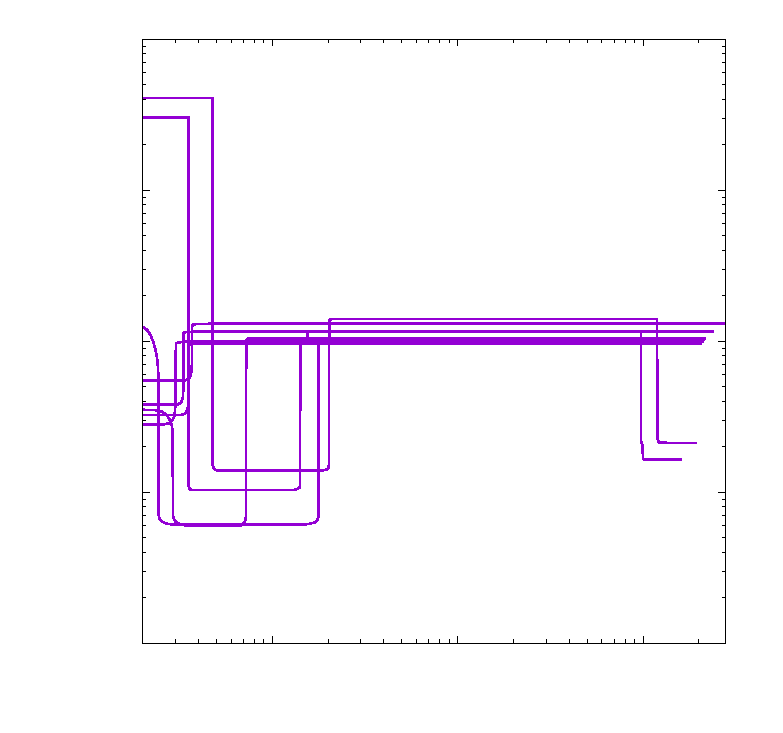
\includegraphics{chq2}}%
    \gplfronttext
  \end{picture}%
\endgroup
 & % GNUPLOT: LaTeX picture with Postscript
\begingroup
  \makeatletter
  \providecommand\color[2][]{%
    \GenericError{(gnuplot) \space\space\space\@spaces}{%
      Package color not loaded in conjunction with
      terminal option `colourtext'%
    }{See the gnuplot documentation for explanation.%
    }{Either use 'blacktext' in gnuplot or load the package
      color.sty in LaTeX.}%
    \renewcommand\color[2][]{}%
  }%
  \providecommand\includegraphics[2][]{%
    \GenericError{(gnuplot) \space\space\space\@spaces}{%
      Package graphicx or graphics not loaded%
    }{See the gnuplot documentation for explanation.%
    }{The gnuplot epslatex terminal needs graphicx.sty or graphics.sty.}%
    \renewcommand\includegraphics[2][]{}%
  }%
  \providecommand\rotatebox[2]{#2}%
  \@ifundefined{ifGPcolor}{%
    \newif\ifGPcolor
    \GPcolortrue
  }{}%
  \@ifundefined{ifGPblacktext}{%
    \newif\ifGPblacktext
    \GPblacktexttrue
  }{}%
  % define a \g@addto@macro without @ in the name:
  \let\gplgaddtomacro\g@addto@macro
  % define empty templates for all commands taking text:
  \gdef\gplbacktext{}%
  \gdef\gplfronttext{}%
  \makeatother
  \ifGPblacktext
    % no textcolor at all
    \def\colorrgb#1{}%
    \def\colorgray#1{}%
  \else
    % gray or color?
    \ifGPcolor
      \def\colorrgb#1{\color[rgb]{#1}}%
      \def\colorgray#1{\color[gray]{#1}}%
      \expandafter\def\csname LTw\endcsname{\color{white}}%
      \expandafter\def\csname LTb\endcsname{\color{black}}%
      \expandafter\def\csname LTa\endcsname{\color{black}}%
      \expandafter\def\csname LT0\endcsname{\color[rgb]{1,0,0}}%
      \expandafter\def\csname LT1\endcsname{\color[rgb]{0,1,0}}%
      \expandafter\def\csname LT2\endcsname{\color[rgb]{0,0,1}}%
      \expandafter\def\csname LT3\endcsname{\color[rgb]{1,0,1}}%
      \expandafter\def\csname LT4\endcsname{\color[rgb]{0,1,1}}%
      \expandafter\def\csname LT5\endcsname{\color[rgb]{1,1,0}}%
      \expandafter\def\csname LT6\endcsname{\color[rgb]{0,0,0}}%
      \expandafter\def\csname LT7\endcsname{\color[rgb]{1,0.3,0}}%
      \expandafter\def\csname LT8\endcsname{\color[rgb]{0.5,0.5,0.5}}%
    \else
      % gray
      \def\colorrgb#1{\color{black}}%
      \def\colorgray#1{\color[gray]{#1}}%
      \expandafter\def\csname LTw\endcsname{\color{white}}%
      \expandafter\def\csname LTb\endcsname{\color{black}}%
      \expandafter\def\csname LTa\endcsname{\color{black}}%
      \expandafter\def\csname LT0\endcsname{\color{black}}%
      \expandafter\def\csname LT1\endcsname{\color{black}}%
      \expandafter\def\csname LT2\endcsname{\color{black}}%
      \expandafter\def\csname LT3\endcsname{\color{black}}%
      \expandafter\def\csname LT4\endcsname{\color{black}}%
      \expandafter\def\csname LT5\endcsname{\color{black}}%
      \expandafter\def\csname LT6\endcsname{\color{black}}%
      \expandafter\def\csname LT7\endcsname{\color{black}}%
      \expandafter\def\csname LT8\endcsname{\color{black}}%
    \fi
  \fi
    \setlength{\unitlength}{0.0500bp}%
    \ifx\gptboxheight\undefined%
      \newlength{\gptboxheight}%
      \newlength{\gptboxwidth}%
      \newsavebox{\gptboxtext}%
    \fi%
    \setlength{\fboxrule}{0.5pt}%
    \setlength{\fboxsep}{1pt}%
\begin{picture}(7200.00,6720.00)%
    \gplgaddtomacro\gplbacktext{%
      \csname LTb\endcsname%%
      \put(1078,704){\makebox(0,0)[r]{\strut{}\Large $10^{1}$}}%
      \put(1078,2153){\makebox(0,0)[r]{\strut{}\Large $10^{2}$}}%
      \put(1078,3601){\makebox(0,0)[r]{\strut{}\Large $10^{3}$}}%
      \put(1078,5050){\makebox(0,0)[r]{\strut{}\Large $10^{4}$}}%
      \put(1078,6499){\makebox(0,0)[r]{\strut{}\Large $10^{5}$}}%
      \put(2454,484){\makebox(0,0){\strut{}\Large$10$}}%
      \put(4233,484){\makebox(0,0){\strut{}\Large$100$}}%
      \put(6013,484){\makebox(0,0){\strut{}\Large$1000$}}%
    }%
    \gplgaddtomacro\gplfronttext{%
      \csname LTb\endcsname%%
      \put(198,3601){\rotatebox{-270}{\makebox(0,0){\strut{}\Large$N (\times 10^3)$}}}%
      \put(4006,154){\makebox(0,0){\strut{}\Large Time ($\times 10^3$ generations)}}%
    }%
    \gplbacktext
    \put(0,0){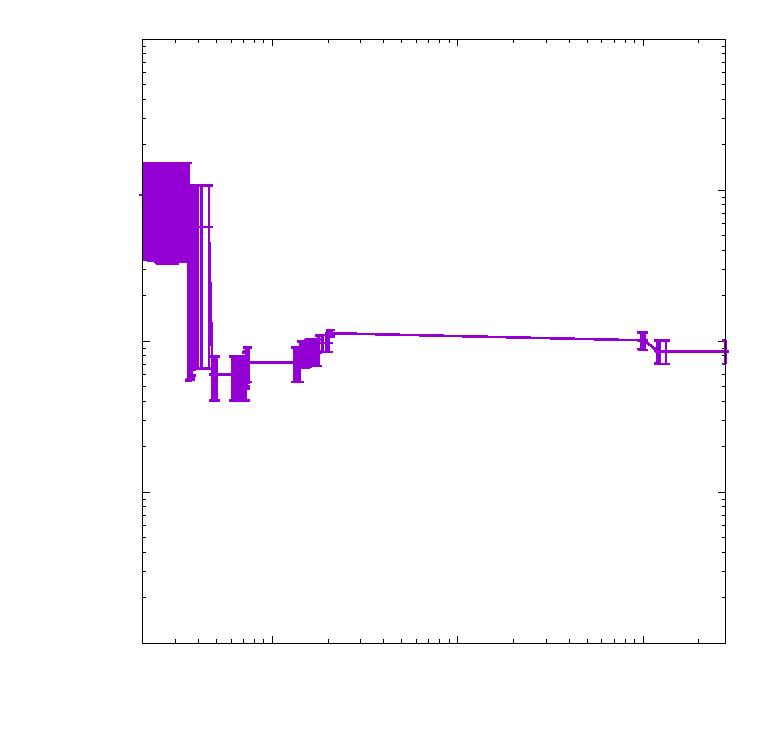
\includegraphics{chq3}}%
    \gplfronttext
  \end{picture}%
\endgroup

      \end{tabular}
    }
  \end{center}
  \caption{Medians of eight bootstrapped runs of \ty{epos2plot} on the
    Chq population of \textit{D. pulex} (\textbf{A}), mean$\pm$SEM of
    that plot.}\label{fig:chq}
\end{figure}


\bibliography{ref}
\end{document}

